\documentclass{article}
\usepackage{amssymb}
\usepackage{amsmath}
\usepackage{centernot}
\usepackage{scalerel}
\usepackage{stackengine}
\usepackage{xcolor}
\usepackage{circuitikz}
\usepackage{graphicx}
\newcommand\showdiv[1]{\overline{\smash{\hstretch{.5}{)}\mkern-3.2mu\hstretch{.5}{)}}#1}}
\newcommand\ph[1]{\textcolor{white}{#1}}


\makeatletter
% we use \prefix@<level> only if it is defined
\renewcommand{\@seccntformat}[1]{%
  \ifcsname prefix@#1\endcsname
    \csname prefix@#1\endcsname
  \else
    \csname the#1\endcsname\quad
  \fi}
% define \prefix@section
\newcommand\prefix@section{}
\newcommand\prefix@subsection{}
\makeatother

\begin{document}

\title{Digital Logic Design: Homework 2}
\author{Joshua Dong}
\date{\today}
\maketitle

Unless otherwise specified, all numbers are decimal.

\section{3.11}
$(A + B' + C + E')(A + B' + D' + E)(B' + C' + D' + E')
\\*
= ((A + B') + (C + E')(D' + E))(B' + C' + D' + E')
\\*
= ((A + B') + (D'E' + CE))(B' + C' + D' + E')
\\*
= (A + B' + D'E' + CE)(B' + C' + D' + E')
\\*
= (A + B' + D'E' + CE)B' + (A + B' + D'E' + CE)C' + (A + B' + D'E' + CE)D' + (A + B' + D'E' + CE)E'
\\*
= AB' + B' + B'D'E' + B'CE + AC' + B'C' + D'E' + AD' + B'D' + D'E' + CED' + AE' + B'E' + D'E'
\\*
= AC' + AE' + B' + CD' + D'E'
$


\section{3.12}
$A'CD'E + A'B'D' + ABCE + ABD = A'B'D' + ABD + BCD'E
\\*
A'CD'E + ABCE + A'B'D' + ABD = A'B'D' + ABD + BCD'E
\\*
CE(A'D' + AB) + A'B'D' + ABD = A'B'D' + ABD + BCD'E
\\*
CE(A'D' + AB + BD') + AB(CE + BD) + A'B'D' + ABD = A'B'D' + ABD + BCD'E
\\*
A'CD'E + ABCE + BCD'E + A'B'D' + ABD = A'B'D' + ABD + BCD'E
\\*
A'CD'E + A'B'D' + (ABD + BCD'E + ABCE) = A'B'D' + ABD + BCD'E
\\*
A'CD'E + A'B'D' + (ABD + BCD'E) = A'B'D' + ABD + BCD'E
\\*
A'B'D' + ABD + BCD'E = A'B'D' + ABD + BCD'E
$
\\
Thus the two sides are equal.


\section{3.12}
\subsection{a)}
$K'L'M + KM'N + KLM + LM'N'
\\*
= K'L'M + KM'N + KLM + LM'N'
\\*
= (K'L'M + K)(K'L'M + M')(K'L'M + N) + L(KM + M'N')
\\*
= (K' + K)(K + L')(M + K)(K' + M')(M' + L')(M + M')(N + K')(N + L')(M + N) + L(KM + M'N')
\\*
= (K + L' + L(KM + M'N'))(M + K + L(KM + M'N'))(K' + M' + L(KM + M'N'))(M' + L' + L(KM + M'N'))(M + M' + L(KM + M'N'))(N + K' + L(KM + M'N'))(N + L' + L(KM + M'N'))(M + N + L(KM + M'N'))
\\*
= (K + L' + M')(K' + L + M')(K + L + M)(L + M + N)(K + M + N')
$
\subsection{e)}
$WXY + WX'Y + WYZ + XYZ'
= (W + X)(W + Y)(W + Z')
$

\section{3.15}
\subsection{a)}
$(K' + M' + N)(K' + M)(L + M' + N')(K' + L + M)(M + N)
\\*
= K'M'N + K'MN' + LMN
$

\section{3.16}
\subsection{b)}
$(KL \oplus M) + M'N'
\\*
= (KLM + (K' + L')M')' + M'N'
\\*
= (K + M + N')(L + M + N')(K' + L' + M')
$

\section{3.19}
\subsection{a)}
$ x + y = x \oplus y \oplus xy
\\*
x + y = (xy + x'y')' \oplus xy
\\*
x + y = ((xy + x'y')'xy + (xy + x'y')(x' + y'))'
\\*
x + y = ((xy + x'y')'xy)'((xy + x'y')(x' + y'))'
\\*
x + y = ((x' + y')(x + y)xy)'((xy + x'y')(x' + y'))'
\\*
x + y = ((x' + y')' + (x + y)' + (x' + y'))((xy + x'y')(x' + y'))'
\\*
x + y = (xy + x'y' + x' + y')((xy + x'y')' + (x' + y')')
\\*
x + y = (xy + x'y' + x' + y')((xy)'(x'y')' + xy)
\\*
x + y = (xy + x' + y')((x' + y')(x + y) + xy)
\\*
x + y = (xy + x' + y')((x' + y' + xy)(x + y + xy))
\\*
x + y = (xy + x' + y')(x' + y' + xy)(x + y)
\\*
x + y = (x' + y' + xy)(x + y)
\\*
x + y = (x' + 1y' + xy + 1x)(x + y)
\\*
x + y = (1)(x + y)
\\*
x + y = x + y
$
\\
Thus the two sides are equal.

\section{3.21}
\subsection{a)}
$BC'D' + ABC' + AC'D + AB'D + A'BD'
= A'BD' + AB'D + ABC'
$
\subsection{b)}
$W'Y' + WYZ + XY'Z + WX'Y
= WX'Y + W'Y' + WXZ
$

\section{3.25}
\subsection{f)}
$A'BCD + A'BC'D + B'EF + CDE'G + A'DEF + A'B'EF
= CDE'G + B'EF + A'BD
$

\section{3.32}
\subsection{c)}
If $A + B = C$, then $A + B + D$ = $C + D$, since the OR operation is a well-defined function.

\section{3.38}
\subsection{a)}
If $x(y + a') = x(y + b')$, then $a = b$ does not hold in general.
\\*
For example, take $x = 0$. No matter what $a$ and $b$ are, both sides will be equal.

\section{4.9}
\subsection{a)}
$F(a, b, c) = abc' + ab'c + ab'c' + a'b'c + a'b'c' = m_0 + m_1 + m_2 + m_3 + m_6$
\subsection{b)}
$F(a, b, c) = M_4M_5M_7$
\subsection{c)}
$F'(a, b, c) = m_4 + m_7$
\subsection{d)}
$F'(a, b, c) = M_0M_1M_2M_3M_6$

\section{4.13}
$ABCD + ABCD' + A'BCD + AB'C'D' + A'B'C'D + A'B'C'D' 
//*
= (ABCD + ABCD') + (ABCD + A'BCD) + (A'B'C'D' + AB'C'D') + (A'B'C'D + A'B'C'D')$,
by associativity and the Idempotent law of boolean addition 
//*
$= ABC + A'B'C' + BCD + B'C'D'$,
by the Uniting Theorem of Addition and commutativity.

This problem was already done to great detail in Lab 1 (pdf attached).
\newpage
\section{4.16}
\subsection{a)}
$z = \sum m(1,2,3,4,5,6,7,8,9,10,11,12,13,14,15)
\\*
y_0 = \sum m(0,2,3,8,9,10,11,12,13,14,15)
\\*
y_1 = \sum m(0,4,5,6,7,8,9,10,11,12,13,14,15)
$
\subsection{b)}
$z = \prod M(0)
\\*
y_0 = \prod M(1,4,5,6,7)
\\*
y_1 = \prod M(1,2,3)
$

\section{4.23}
$F_1F_2 = \prod M(0,4,5,6,7)$, since the product of products is the product of the terms.
\\*
Proof: $\prod M(a_0, a_1, ..., a_n) \cdot
\prod M(b_0, b_1, ..., b_m)
= M_{a_1}M{a_2}...M{a_n}M{b_1}M{b_2}...M{b_m}$.
\\*
$M_{x}M_{y} = M{x}$ when $x = y$, so we can simplify like terms of the product.

\section{4.24}
$F_1 + F_2 = \sum m(1,2,3,7) + \sum m(1,2,3,5,6) = \sum m(1,2,3,5,6) = \prod M(0,4)$,
since the sum of sums is a sum of the terms.
\\*
A general rule is that we can take the intersection of the terms of the maxterm product as the resulting product.
\\*
The proof is similar to the one provided prior. 
$\prod M(a_0, a_1, ..., a_n) +
\prod M(b_0, b_1, ..., b_m)
= m_{c_1} + m{c_2} + ... + m{c_x} + m{d_1} + m{b_2} + ... + m{d_y}$, where $c_i$ is the $i^{th}$ term not in the series of a, and $d_j$ is the $j^{th}$ term not in the series of b.
\\*
$m_{x} + m_{y} = m{x}$ when $x = y$, so we can simplify like terms of the sum.

\section{4.35}
\subsection{a)}
$X = \sum m(1,2,4,7,8,11,13,14)
Y = \sum m(3,5,6,7,9,10,11,12,13,14)
Z = \sum m(15)
$

\subsection{b)}
$X = \prod M(0,3,5,6,9,10,12,15)
Y = \prod M(0,1,2,4,8,15)
Z = \prod M(0,1,2,3,4,5,6,7,8,9,10,11,12,13,14)
$

\section{4.40}
$
\begin{array}{ccc|cccc}
A&B&&S&C
\\\hline
0&0&&0&0\\
0&1&&1&0\\
1&0&&1&0\\
1&1&&0&1
\end{array}
$
\\
\begin{circuitikz} \draw
    (0,1) node[and port] (myand) {}
    (2,3) node[xor port] (myxor) {}
    (myand.in 1) -- (myxor.in 1)
    (myand.in 2) -- (myxor.in 2);
\end{circuitikz}
\\
The output of the AND gate is carry bit and the output of the XOR gate is the sum bit.
The inputs are symmetric.
\\\\
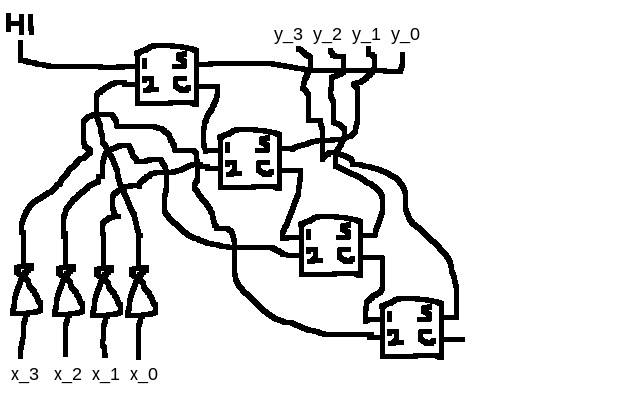
\includegraphics[scale=0.7]{2s}
The unused carry bit could be grounded perhaps.

\end{document}
